\documentclass[a4paper,12pt,twoside]{article}
\usepackage{amsmath}
\usepackage{amssymb}
\usepackage{bm}
\usepackage{booktabs}
\usepackage[small,bf]{caption}
\usepackage{comment}
\usepackage{cuted}
\usepackage[shortlabels]{enumitem}
\usepackage{fancyhdr}
\usepackage{fancybox}
\usepackage{float}
\usepackage[T1]{fontenc}
\usepackage[a4paper,left=1in,right=1in,top=0.25in,bottom=1in,
    headheight=76.33466pt,
    headsep=\dimexpr1in-62.33466pt\relax,
    includehead
]{geometry}
\usepackage{graphicx}
\usepackage{hyperref}
\usepackage[utf8]{inputenc}
% \usepackage{lipsum}
% \usepackage{listings}
% \usepackage{minted}
% \usemintedstyle{tango}
\usepackage{multirow}
\usepackage{parskip}
\usepackage{ragged2e}
\usepackage{setspace}
\usepackage{soul}
% \onehalfspacing
% \usepackage[subrefformat=parens,labelformat=parens]{subfig}
\usepackage{tabularx}
% \usepackage{titling}
\usepackage{xurl}
\usepackage{biblatex}
% \addbibresource{ref.bib}
\usepackage{background}
\backgroundsetup{contents=
\includegraphics{waterprint.jpg}, scale=0.8, opacity=0.1}
\pagestyle{fancy}
\fancyhf{}
\fancyhead[LE,RO]{}
\fancyhead[CE,CO]{
\includegraphics[width=0.7\textwidth]{JILogo.png}}
\fancyhead[RE,LO]{}
\fancyfoot[CE,CO]{\leftmark}
\fancyfoot[CE,CO]{\thepage}
\lfoot{\textit{ECE4810J \textbf{SoC Design} | Fall 2022}}
\renewcommand{\headrulewidth}{1pt}
\renewcommand{\footrulewidth}{1pt}
\definecolor{caption2color}{HTML}{2e5395}
\hypersetup{
    colorlinks=true,
    linkcolor=blue,
    filecolor=magenta,      
    urlcolor=cyan,
    pdfpagemode=FullScreen,
}

\author{Xinfei Guo, Yihua Liu}
\title{ECE4810J FA2021\\ \small Lab \#0 Reading Assignment}
\date{September 3, 2022}

\begin{document}
% \maketitle
\thispagestyle{fancy}

\begin{center}
    \vspace*{0pt}
    \Large{\textbf{ECE4810J SoC Design}}\\
    \vspace*{2pt}
    \large{Fall 2022}\\
    \vspace*{10pt}
    \Large{\textcolor{caption2color}{Lab \#0 Getting to know Xilinx Arty Z7 \& Vivado}}\\
    \normalsize{\hl{Due: 11:59pm Sunday Sept. 18th, 2022}}
    \rule[-5pt]{.97\linewidth}{0.05em}
\end{center}
\begin{FlushRight}
\textit{Please Submit a PDF file on Canvas}
\end{FlushRight}

\section{Xilinx Arty Z7 Platform}
The Arty Z7 is a ready-to-use development platform designed around the Zynq-7000™ All Programmable System-on-Chip (AP SoC) from Xilinx. It will be used as the main SoC platform for this course throughout the semester. In this assignment, you will be assigned to read several documents about this board and the SoC. Please answer the questions below and submit through canvas. Note that this is an \hl{individual} lab assignment.

References:
\begin{enumerate}
    \item Read about Arty Z7 reference manual \url{https://digilent.com/reference/programmable-logic/arty-z7/start}
    \item Zynq datasheet (go to Canvas > Files > Reading Materials > Zynq > ds187-XC7Z010-XC7Z020-Data-Sheet.pdf\\or\\ \url{https://jicanvas.com/courses/43/files/594}
    \item The Zynq Book (go to Canvas > Files > Reading Materials > Zynq >\\The\_Zynq\_Book\_ebook\_3.pdf\\or\\\url{http://www.zynqbook.com/})
\end{enumerate}

Questions:
\begin{enumerate}
    \item (10\%)What are the benefits of having Programmable logic on Zynq?
    \item (20\%) How many cores does Zynq-7000 have? What are the names of those cores? What does the memory hierarchy look like? What is the main CPU frequency? 
    \item (15\%) Please list the main interfaces of the Zynq-7000 AP SoC device.
    \item (5\%) How is the Arty Z7 board powered?
    \item (10\%) What is the Quad SPI Flash? What is its usage on this board?
    \item (10\%) What is DDR Memory? What is its usage?
    \item (20\%) What are the main custom IP blocks creation methods Xilinx provides?
    \item (10\%) What is High-Level Synthesis (HLS)? What are the motivations behind HLS? 
\end{enumerate}
\newpage
\section{Installing Vivado Vitis for the first time}
Xilinx Vitis Installation Guide: \href{https://digilent.com/reference/programmable-logic/guides/installing-vivado-and-vitis}{Installing Vivado, Vitis, and Digilent Board Files}
\begin{itemize}
    \item Visit \url{https://china.xilinx.com/support/download/index.html/content/xilinx/zh/downloadNav/vitis.html}.
    \item Uninstall previous versions of Vitis or Vivado. Download Xilinx Unified Installer 2022.1 SFD (TAR/GZIP - 73.81 GB). Extract the zipped file.
    \item Under folder \texttt{Xilinx\_Unified\_2022.1\_0420\_0327}, run \texttt{xsetup.exe}:
    \begin{figure}[H]
        \centering
        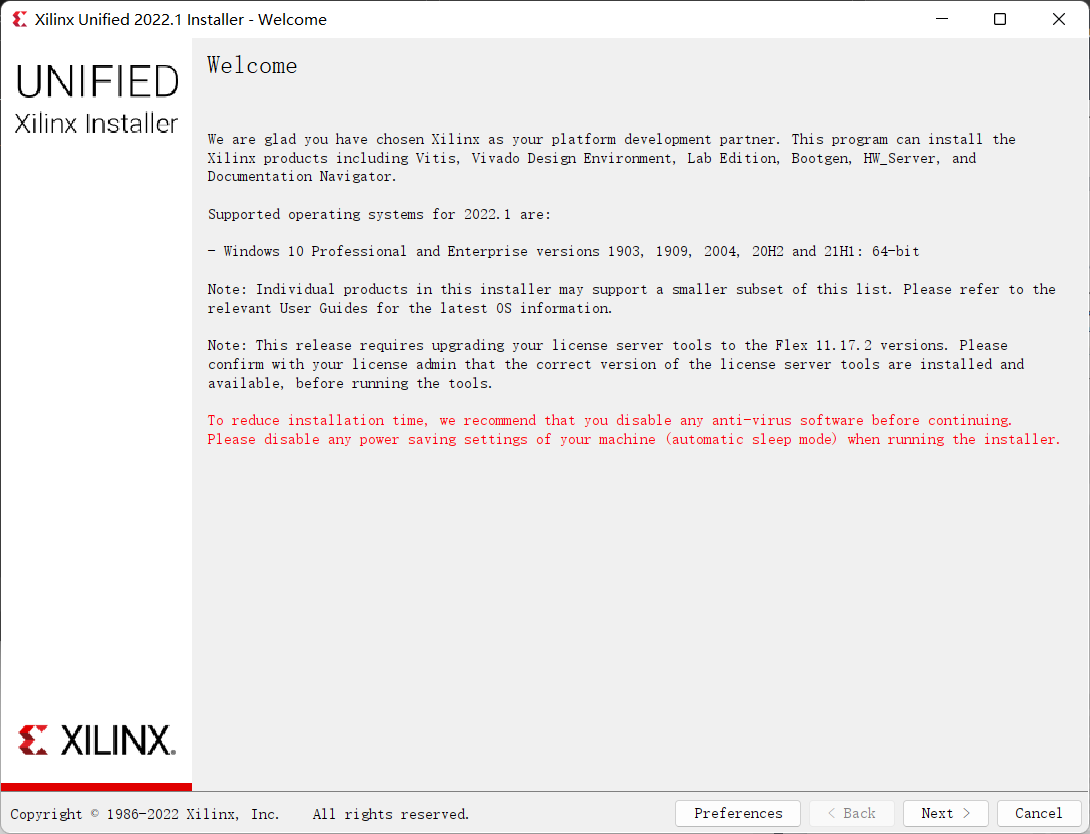
\includegraphics[width=0.65\textwidth]{1.png}
    \end{figure}
    \item Click Next:
    \begin{figure}[H]
        \centering
        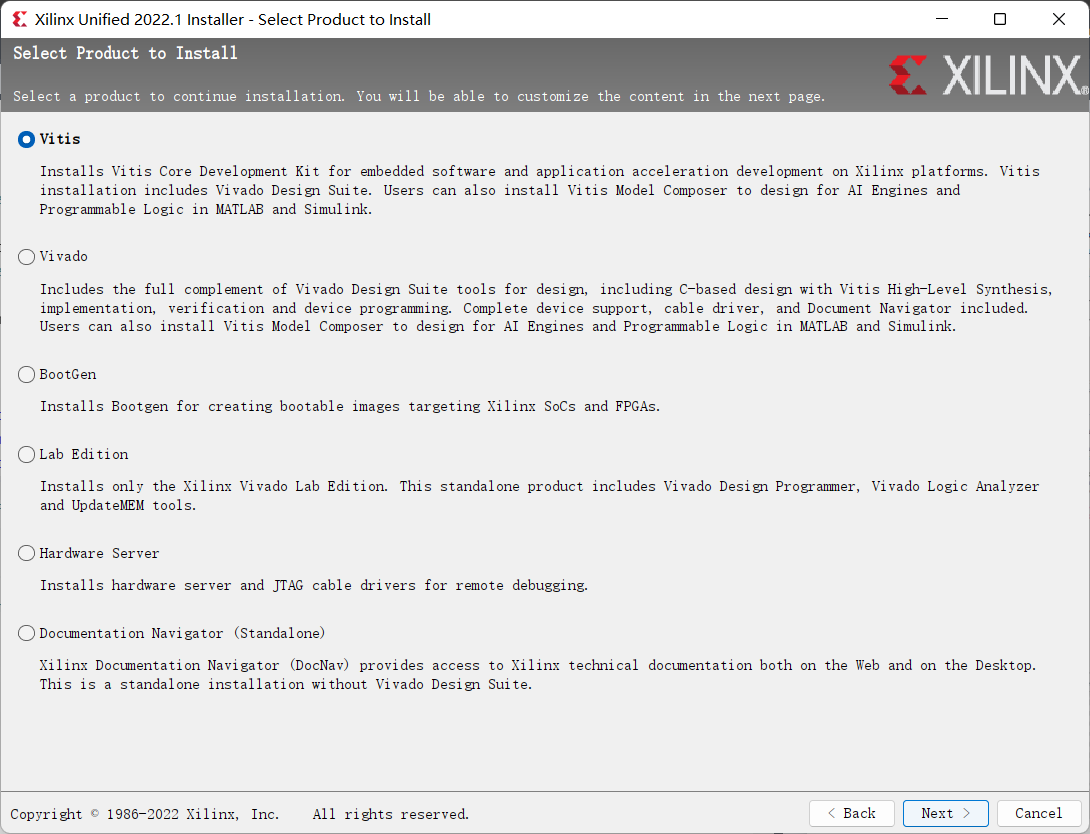
\includegraphics[width=0.65\textwidth]{2.png}
    \end{figure}
    \item Click Next. Select all (for Devices for Custom Platforms, at least select SoCs and UltraScale+):
    \begin{figure}[H]
        \centering
        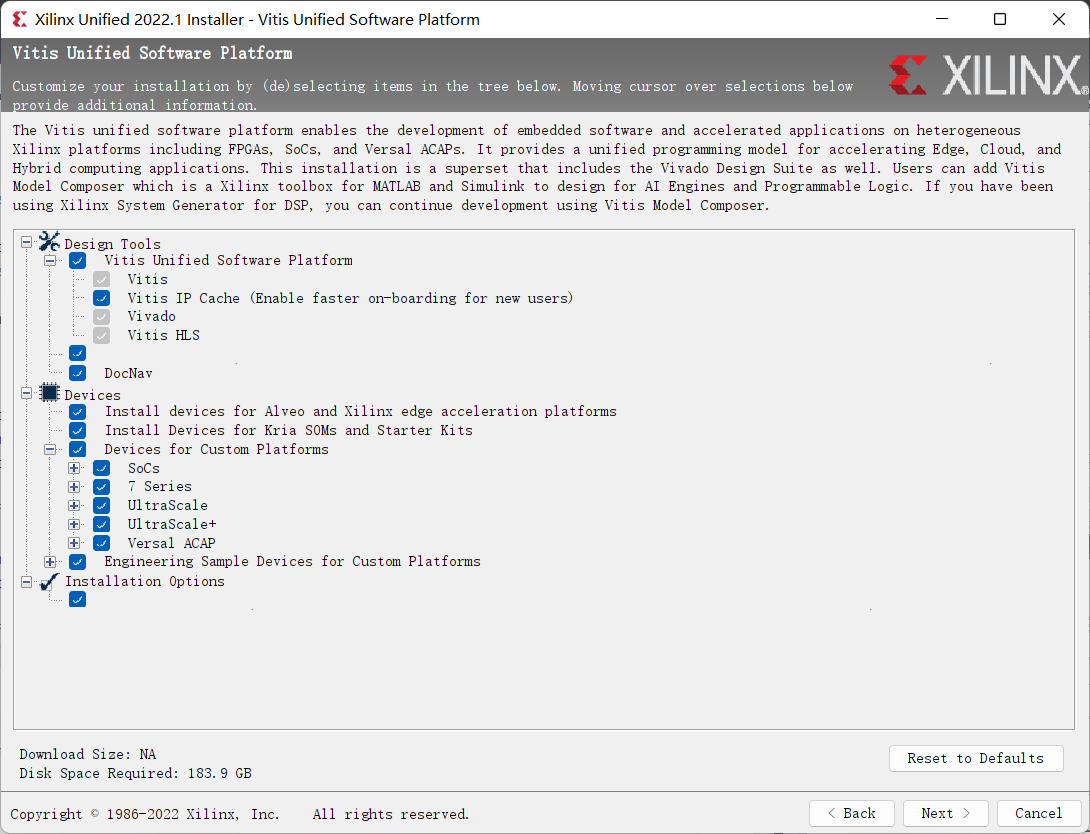
\includegraphics[width=0.8\textwidth]{3.png}
    \end{figure}
    \item Click Next. Check "I Agree" for all:
    \begin{figure}[H]
        \centering
        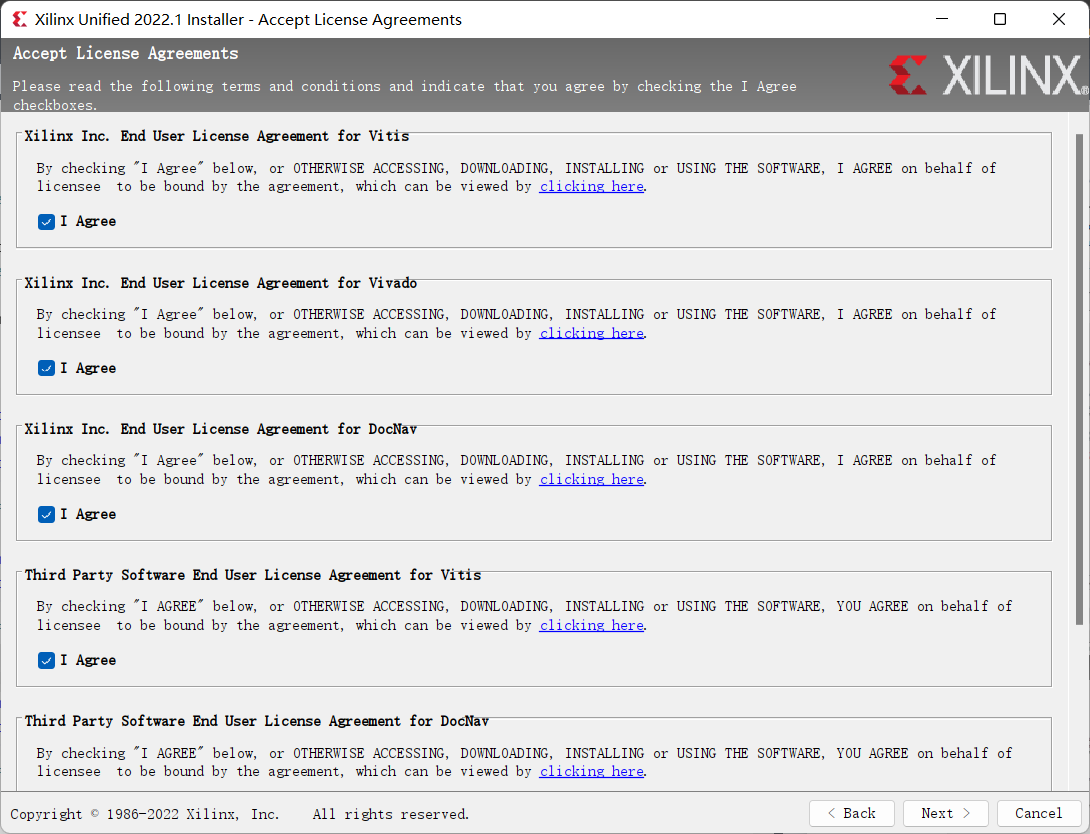
\includegraphics[width=0.8\textwidth]{4.png}
    \end{figure}
    \item Select the installation directory:
    \begin{figure}[H]
        \centering
        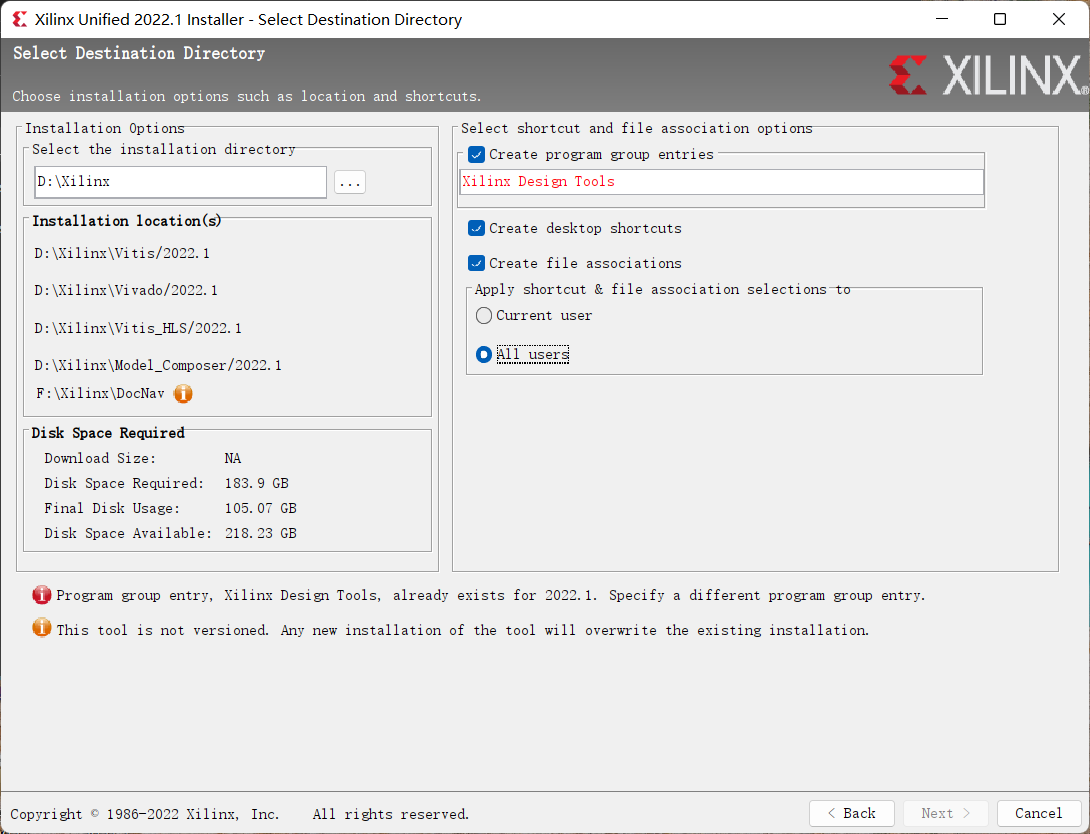
\includegraphics[width=0.85\textwidth]{5.png}
    \end{figure}
    \item Click Install:
    \begin{figure}[H]
        \centering
        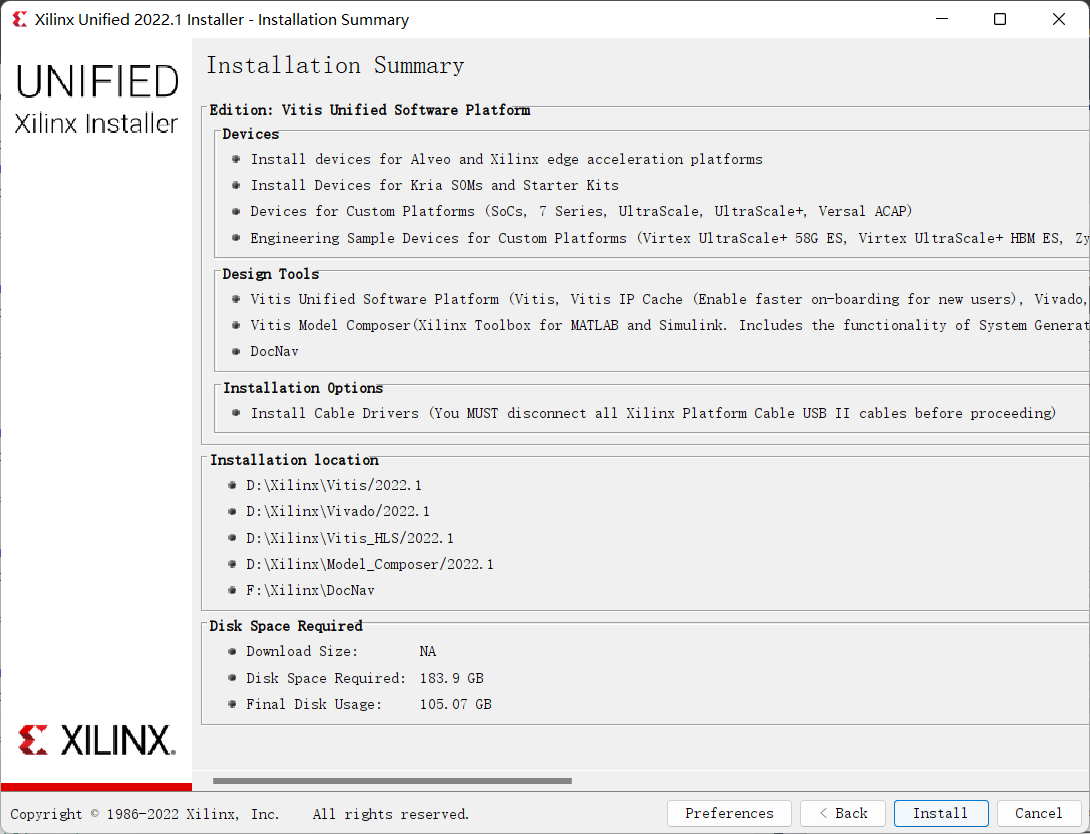
\includegraphics[width=0.85\textwidth]{6.png}
    \end{figure}
    \item Download Xilinx Unified 2022.1.2 : All OS installer Single-File Download (TAR/GZIP - 56.25 GB). Extract the zipped file.
    \item Under folder \texttt{Xilinx\_Vivado\_Vitis\_Update\_2022.1.2\_0806\_0242}, run \texttt{xsetup.exe}.
    \item Install the update.
    \item Clone the board files repository from \href{https://github.com/Digilent/vivado-boards}{Digilent/vivado-boards}.
    \begin{figure}[H]
        \centering
        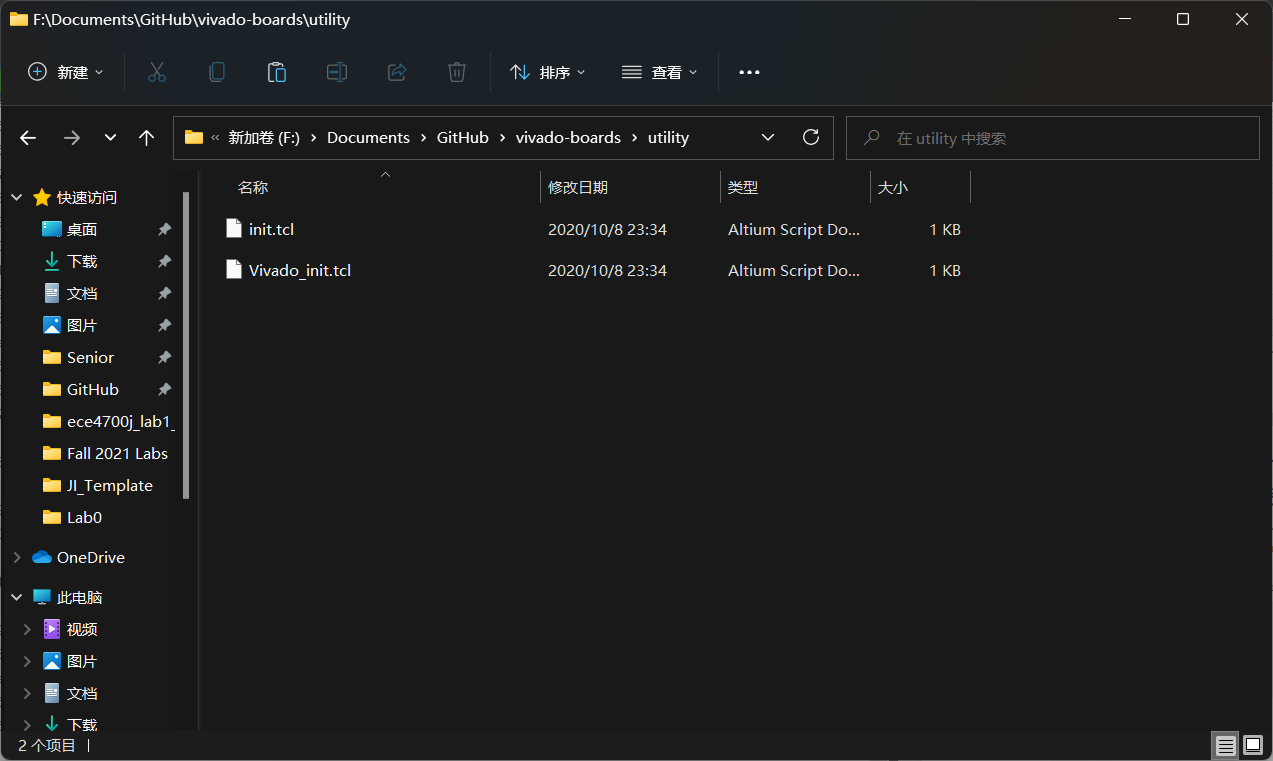
\includegraphics[width=0.9\textwidth]{7.png}
    \end{figure}
    \item Copy \texttt{vivado-boards/utility/Vivado\_init.tcl} and paste it into the\\ \texttt{\%APPDATA\%/Xilinx/Vivado/} directory.
    \begin{figure}[H]
        \centering
        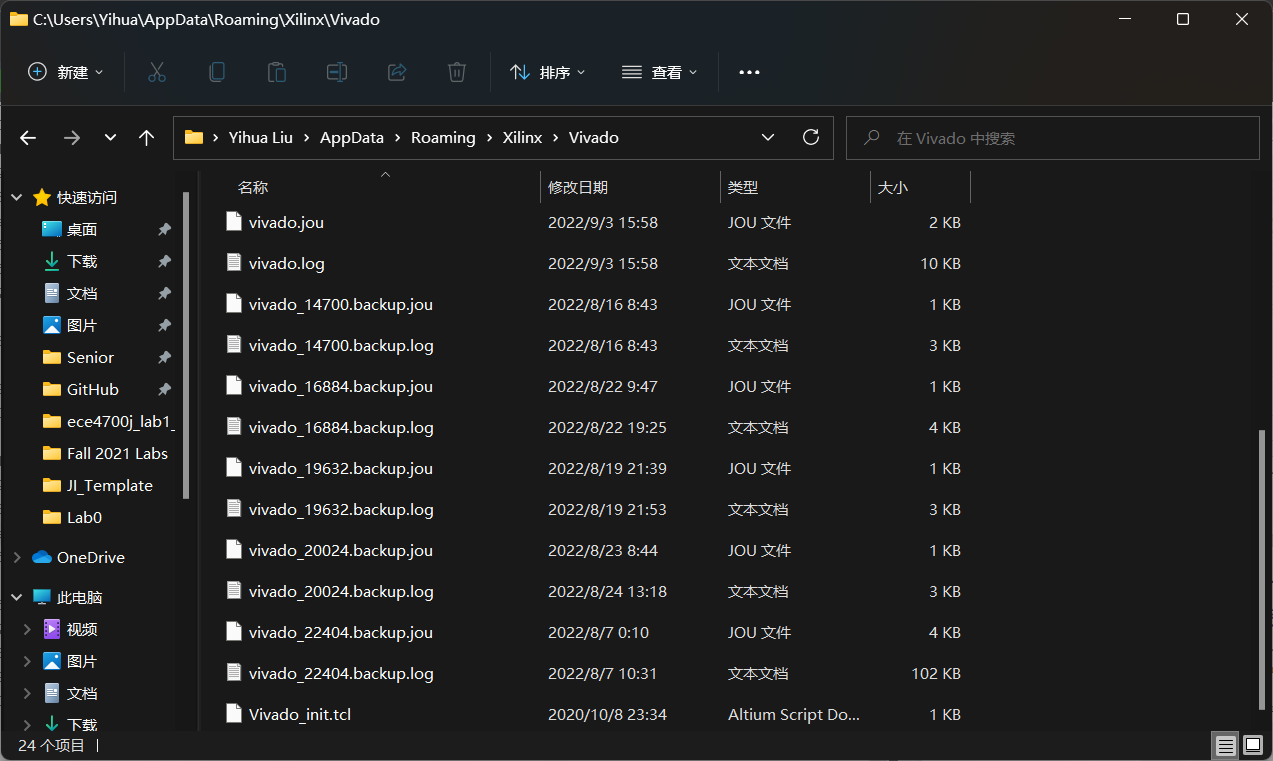
\includegraphics[width=0.9\textwidth]{8.png}
    \end{figure}
    \item Open the copied init script in a text editor. Change the text <extracted path> in the script to the path to the extracted vivado-boards folder. Save and close the file.
    \begin{figure}[H]
        \centering
        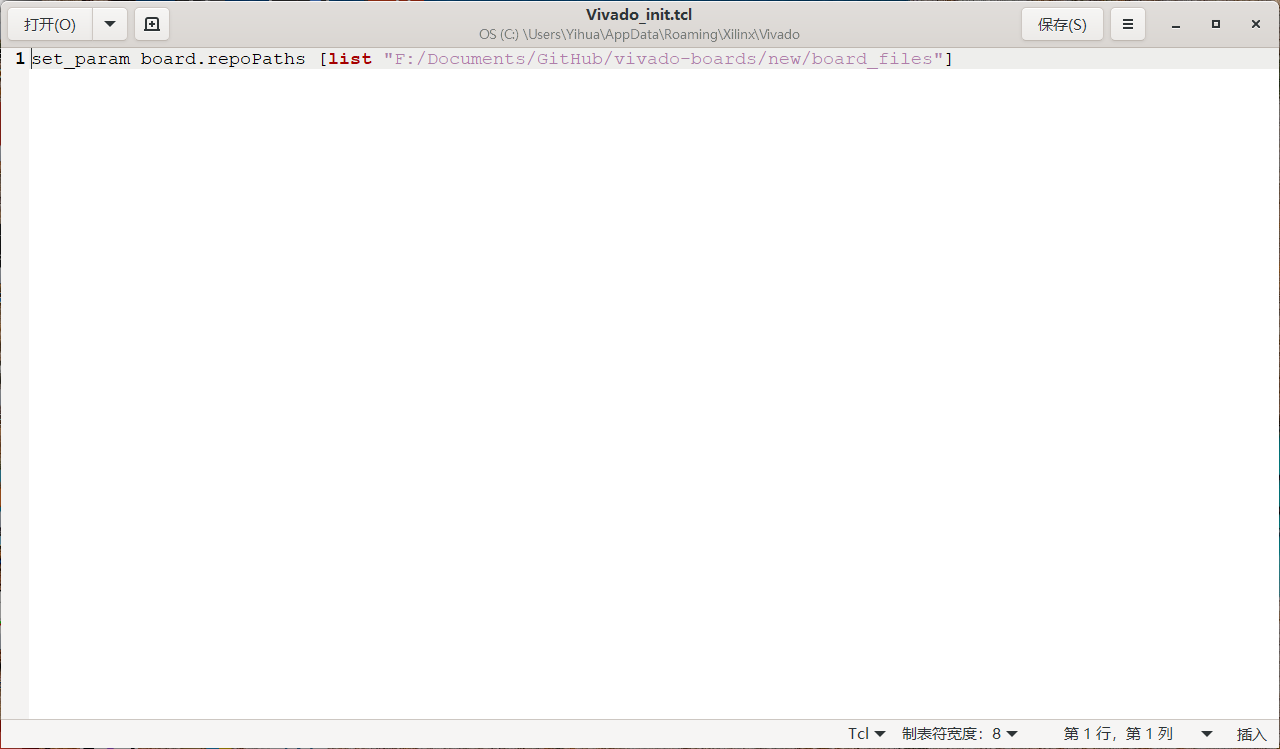
\includegraphics[width=1\textwidth]{9.png}
    \end{figure}
    \item Check in Vivado:
    \begin{figure}[H]
        \centering
        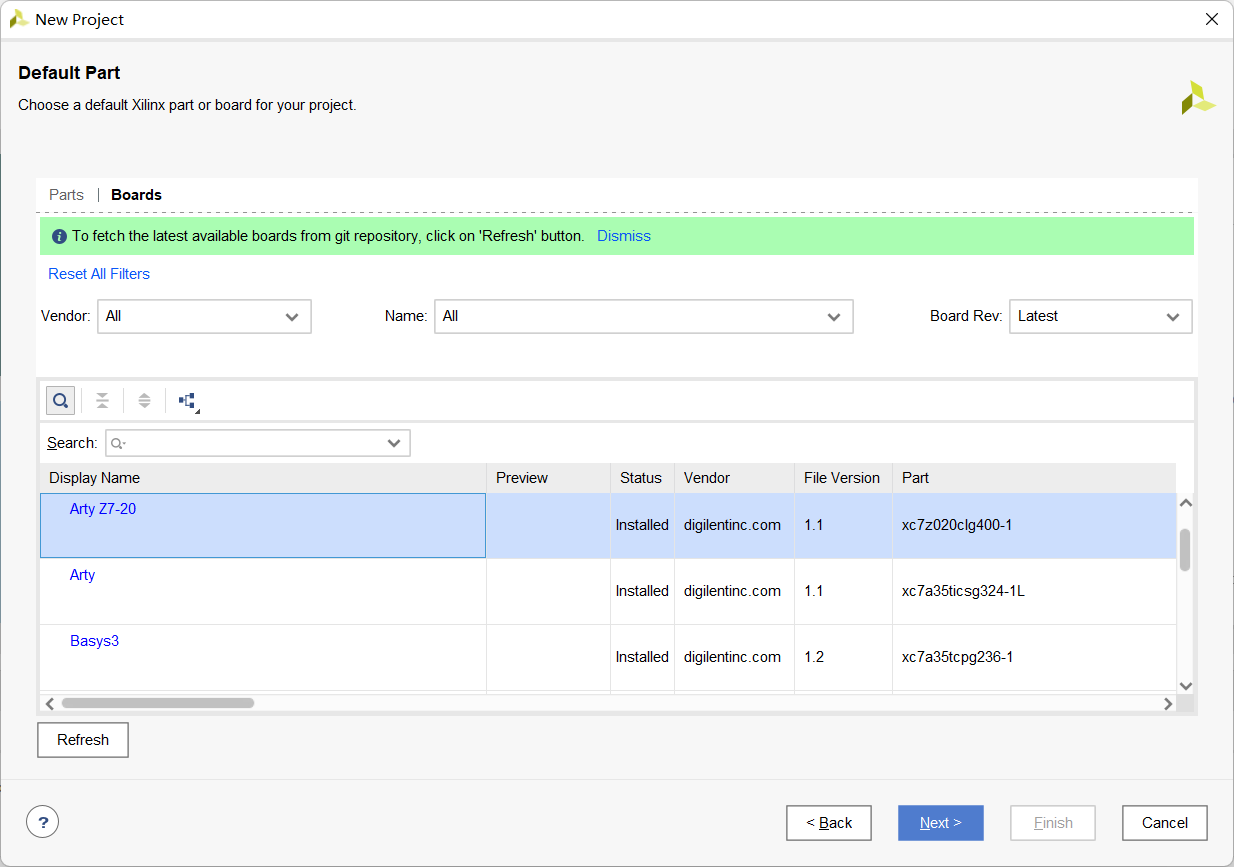
\includegraphics[width=1\textwidth]{10.png}
    \end{figure}
\end{itemize}

% \printbibliography
\end{document}

